\chapter{Single dimension model combination\label{sec:combination}}\thispagestyle{empty}

In chapter \ref{sec:singleDimension}, the construction of single dimension models is discussed.
These models extimate the segmentation masks of $352 mm\times 352 mm$ patches of scan volume slices along one of the three main axis.
In this chapter, the results of these single dimension models are combined to form a \textit{pseudo} mask that is subsequently used as labelling to train the final segmentation network.
Details regarding this combination procedure are given on page \pageref{sec:combinationProcedure}.
Interesting to note in this procedure is that the evaluation metric of these obtained segmentation masks is improved in each of these steps.
The pseudo mask volume performs better than the single dimension model results and the final model trained on the pseudo masks performs better than the pseudo mask itself. 

\begin{SCtable}[\sidecaptionrelwidth][h]

    \begin{tabular}{l|lll}
        \hline
        \textbf{\begin{tabular}[c]{@{}l@{}}Slice \\ direction\end{tabular}} &
          \textbf{Transverse} &
          \textbf{Coronal} &
          \textbf{Sagittal} \\ \hline
        \begin{tabular}[c]{@{}l@{}}Context\\ Slices {[}mm{]}\end{tabular}           & 1      & 1      & 1      \\ \cline{1-1}
        \begin{tabular}[c]{@{}l@{}}Points per\\ class instance\end{tabular}         & 1      & 1      & 1      \\ \cline{1-1}
        \begin{tabular}[c]{@{}l@{}}Background \\ points\end{tabular}                & 5      & 3      & 3      \\ \cline{1-1}
        Dataset &
          \begin{tabular}[c]{@{}l@{}}PLoS\\ xVertSeg\\ USiegen\\ MyoSegmenTUM\end{tabular} &
          \multicolumn{2}{l}{\begin{tabular}[c]{@{}l@{}}xVertSeg\\ USiegen\\ MyoSegmenTUM\end{tabular}} \\ \cline{1-1}
        \begin{tabular}[c]{@{}l@{}}Segmentation\\ classes\end{tabular}              & 2      & 6      & 6      \\ \cline{1-1}
        \begin{tabular}[c]{@{}l@{}}score \\ $dice_{wi}$\end{tabular}              & 0.46   & 0.38   & 0.38   \\ \hline
        \begin{tabular}[c]{@{}l@{}}score \\ $dice_{wi}$\\ combination\end{tabular} & \multicolumn{3}{c}{0.51} \\ \hline
        \end{tabular}
    \caption{Combination of three point supervised models with algorithm \ref{alg:combination}. 
    These models were constructed with a fixed number of background points and a fixed number of class labels per class instance.
    This test indicates that the segmentation mask obtained from the result of single dimension models with algorithm \ref{alg:combination} allows to obtain a new segmentation mask with a higher metric score, the pseudo masks.
    The inverse weighted dice scores are evaluated on the cross validation set, this causes the difference with the values in figure \ref{fig:points_influence}. \label{tab:combination_1}
    }

\end{SCtable}
\par{
    In table \ref{tab:combination_1}, the segmentation quality is calculated on the validation set.
    Since there are two hyperparameters (the number of denoise iterations and the number of erosion iterations) to optimise in the combination algorithm \ref{alg:combination}, 
    the algorithm is evaluated with a matrix of these hyperparameters to choose the optimal hyperparameter set to construct the pseudo masks for the test set.
    In figure \ref{fig:hyperparameter_combination_1}, this obtimization procedure is illustrated.
    The optimal hyperparameter set in this case was 2 denoise iterations and 1 erosion iteration.
}
\marginpar{
        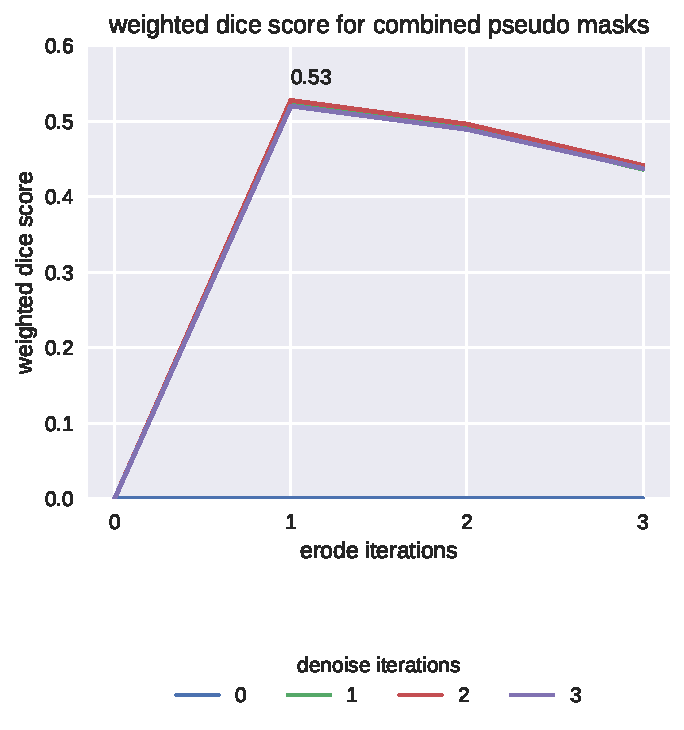
\includegraphics[width=5cm]{images/combination_optimization_1.pdf}
        \captionof{figure}{Illustration of the hyperparameter optimization procedure for the combination detailed in \ref{tab:combination_1}}
        \label{fig:hyperparameter_combination_1}
    }
\par{
    The result of this procedure is illustrated in figures \ref{fig:comb1_1}, \ref{fig:comb1_2} and \ref{fig:comb1_3}.
    These images illustrate that the result of the combination procedure is an improvement compared to the results of the individual models.
}   
\par{
    The procedure described in the last two chapters now allows to train a network with only point annotated labels by using the results of the pseudo mask volume.
    Mind however that the results in chapter \ref{sec:singleDimension} and the results combined in this chapter were obtained with a different set of point annotations for each dimension.
    This was done to make comparison possible. The next chapter discusses a more realistic scenario.
}

\begin{SCfigure}[][htb]
    \centering
    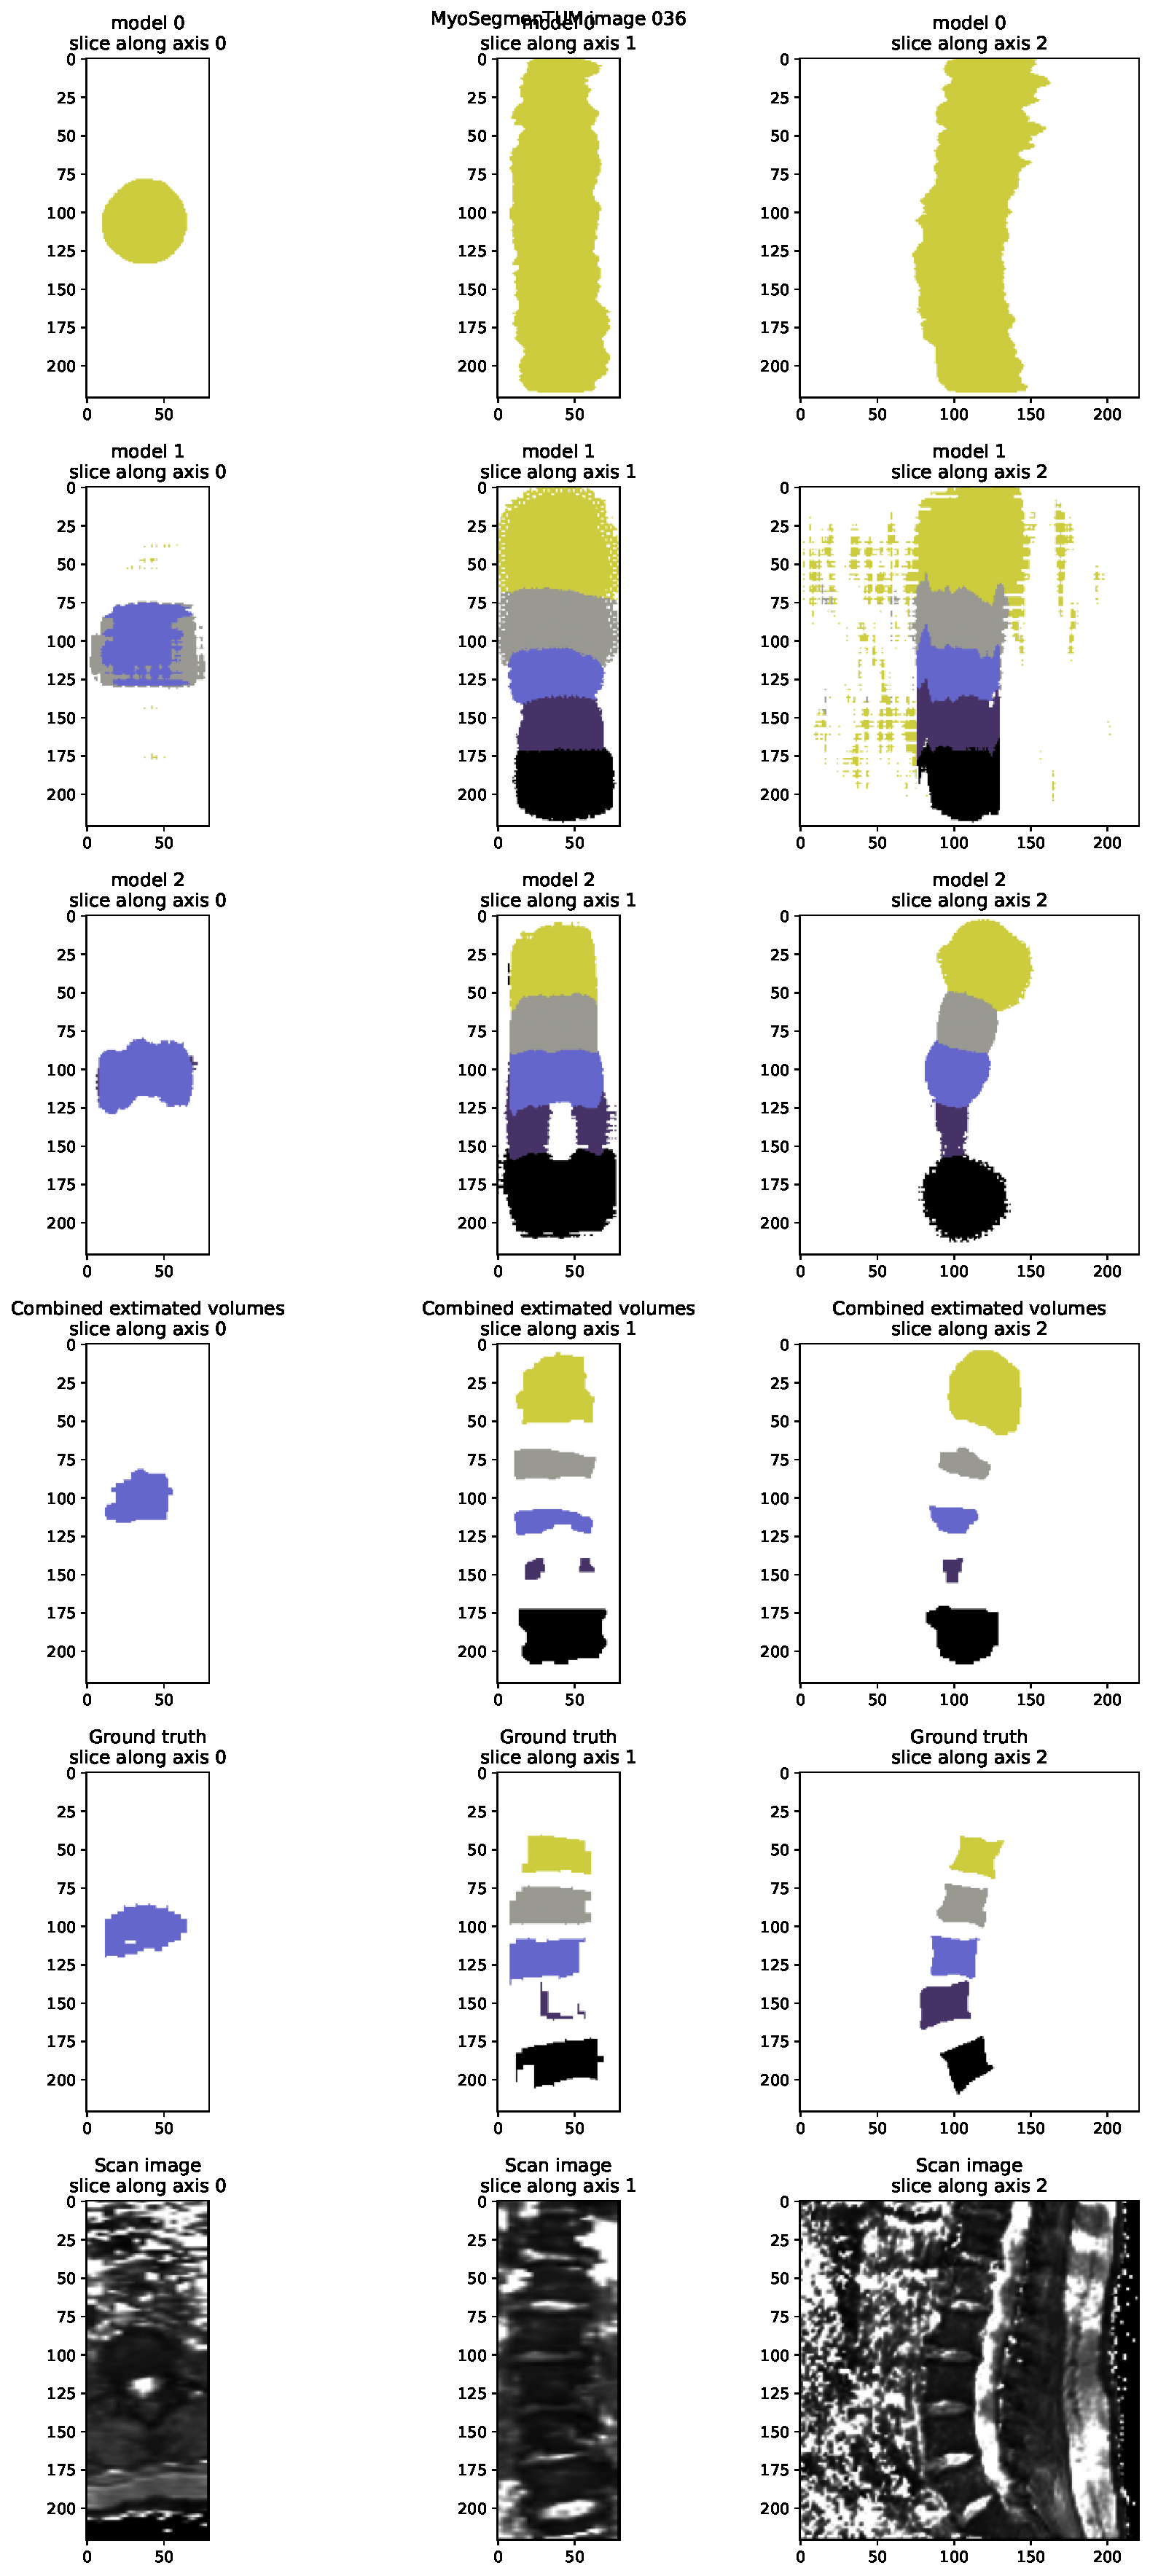
\includegraphics[width=.95\textwidth]{images/comb1_denoise2_erode1_MyoSegmenTUM_036.pdf}
    \caption{
        Result of the combination of the three single dimension model results for volume MyoSegmenTUM nr 36.
        The colours indicate the vertebra classes. Only one semantic class is estimated in the first row, illustrating the model trained on transversal slices.
        On the first three rows, slices of the resulting segmentations from the single dimension models are shown. 
        It is clear these masks contain some artefacts and are not always in agreement with each other.
        On the fourth row, the result after mask combination and morphological smoothing is shown. 
        This corresponds more closely to the ground truth mask, shown on the fifth row.
        This final mask, shown on the fourth row, will be used as a pseudo mask to approximate the unknown ground truth mask.
        In the last row, the corresponding images are shown. 
        \protect\newline\noindent Colour legend: \newline
\noindent\mycircle{colL1}  L1 %\newline 
\hspace{2mm}\mycircle{colL2}  L2 %\newline 
\hspace{2mm}\mycircle{colL3}  L3 %\newline 
\hspace{2mm}\mycircle{colL4}  L4 %\newline 
\hspace{2mm}\mycircle{colL5}  L5
        \label{fig:comb1_1}
    }
\end{SCfigure}
\begin{SCfigure}[][htb]
    \centering
    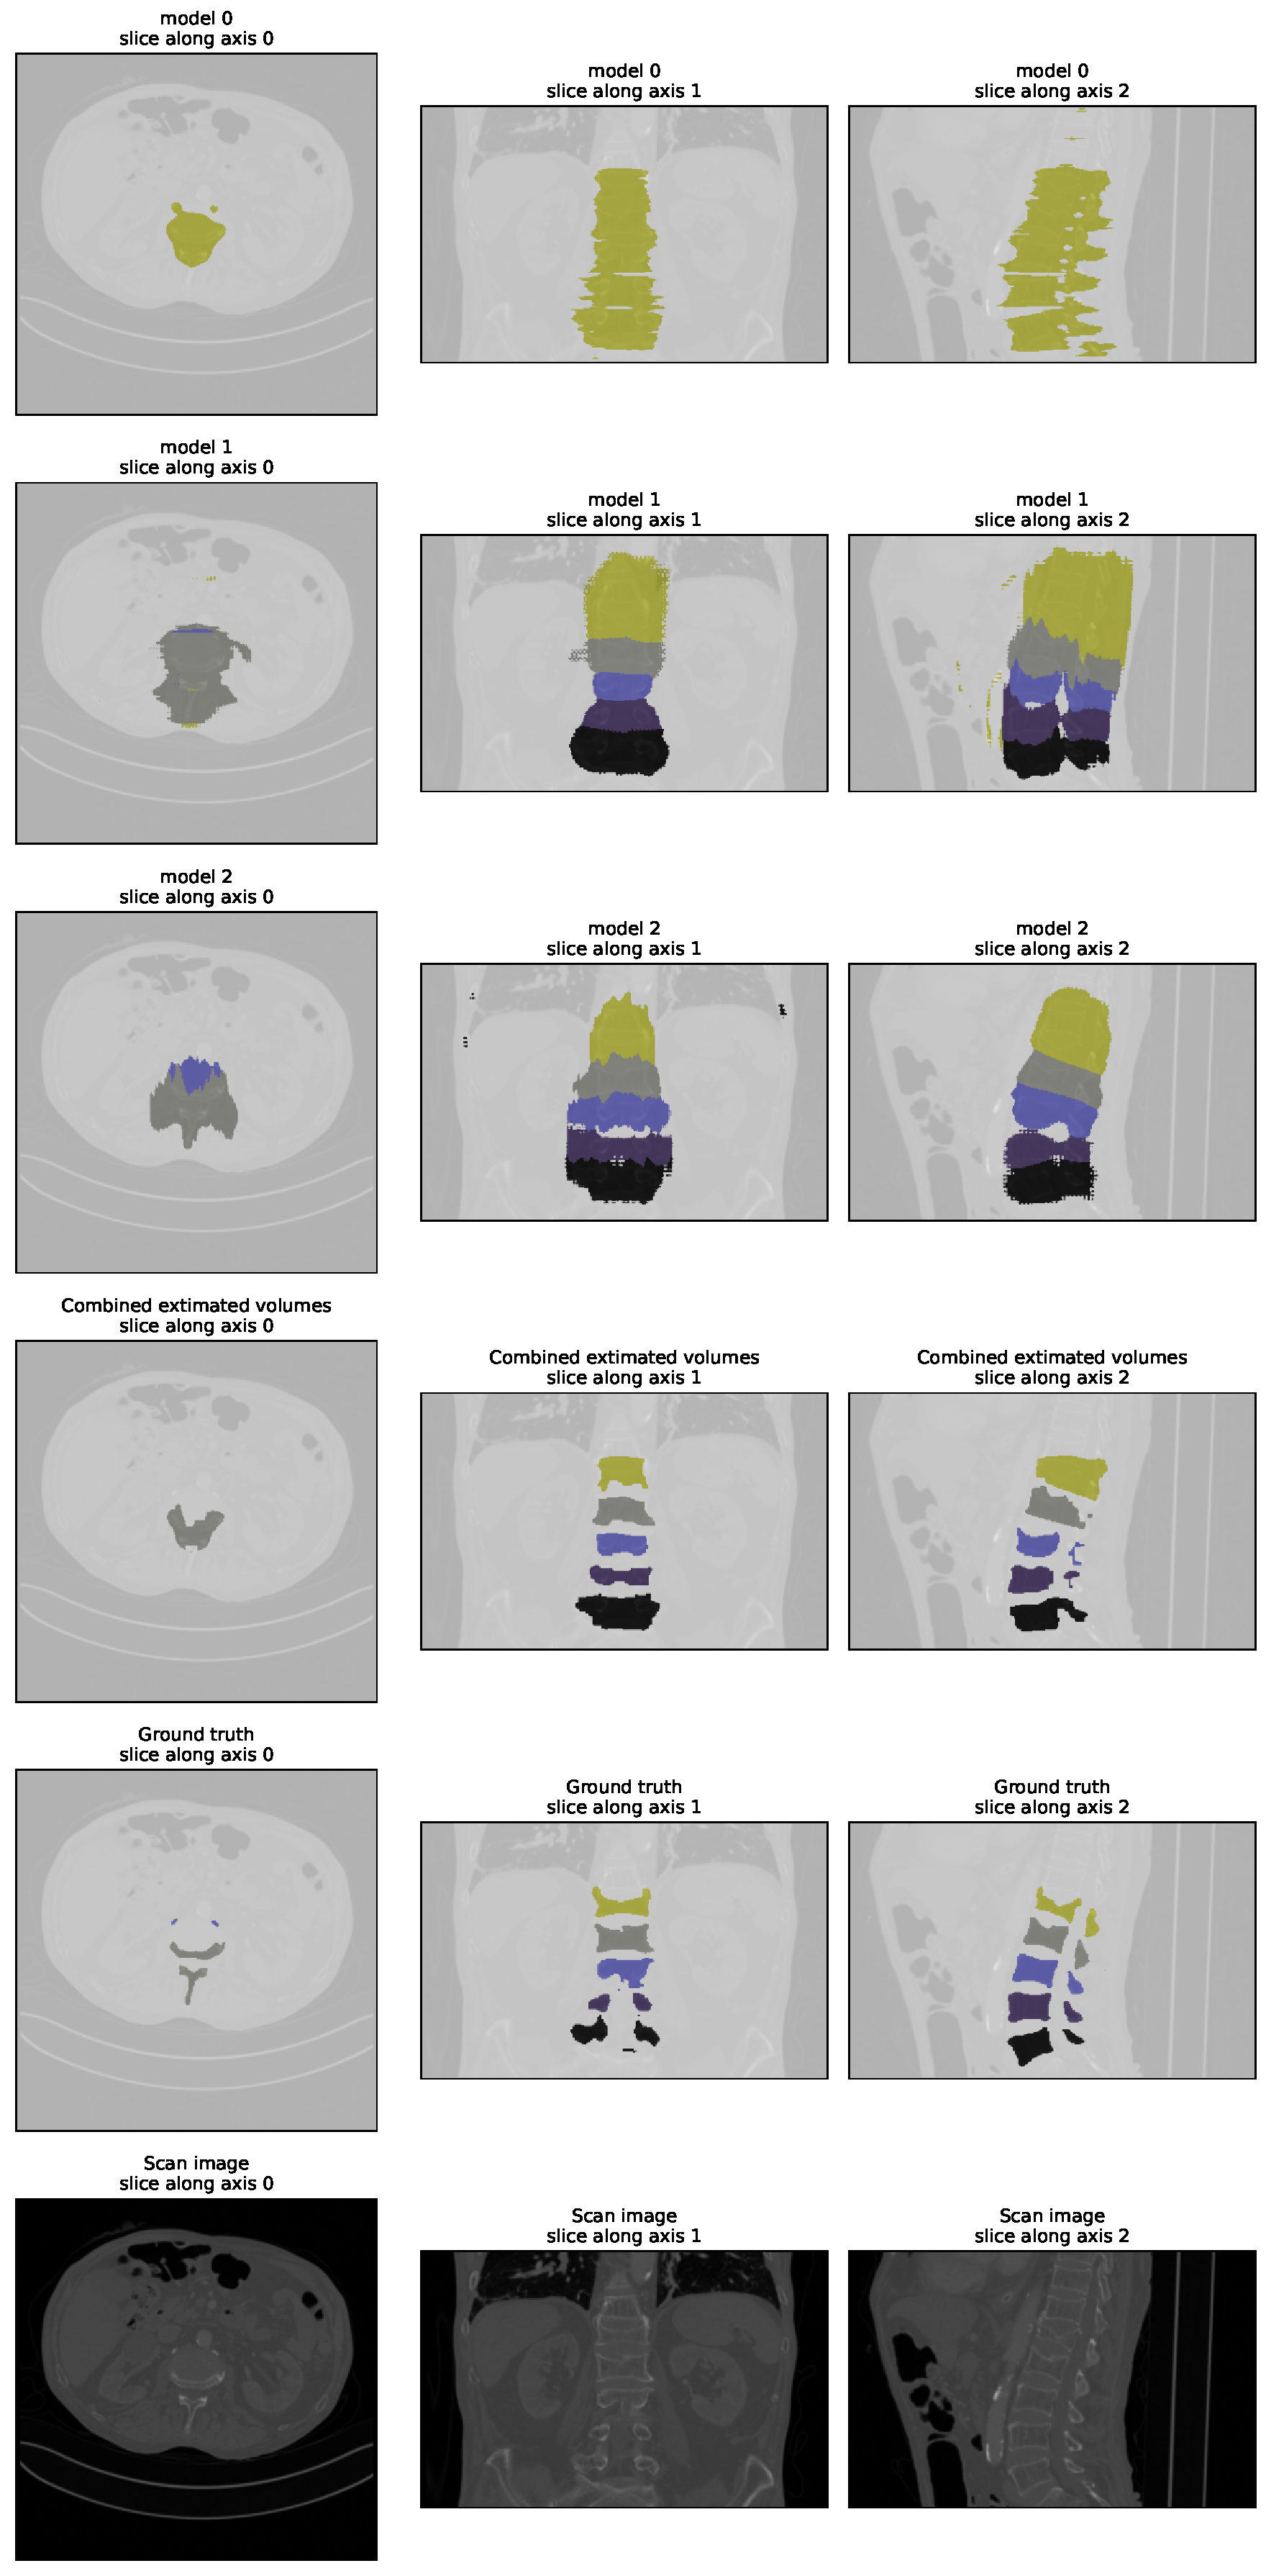
\includegraphics[width=.95\textwidth]{images/comb1_denoise2_erode1_xVertSeg_009.pdf}
    \caption{
        Result of the combination of the three single dimension model results for volume xVertSeg 009. The layout of this picture is identical to figure \ref{fig:comb1_1}.
        \protect\newline\noindent Colour legend: \newline
\noindent\mycircle{colL1}  L1 %\newline 
\hspace{2mm}\mycircle{colL2}  L2 %\newline 
\hspace{2mm}\mycircle{colL3}  L3 %\newline 
\hspace{2mm}\mycircle{colL4}  L4 %\newline 
\hspace{2mm}\mycircle{colL5}  L5
        \label{fig:comb1_2}
    }
\end{SCfigure}
\begin{SCfigure}[][htb]
    \centering
    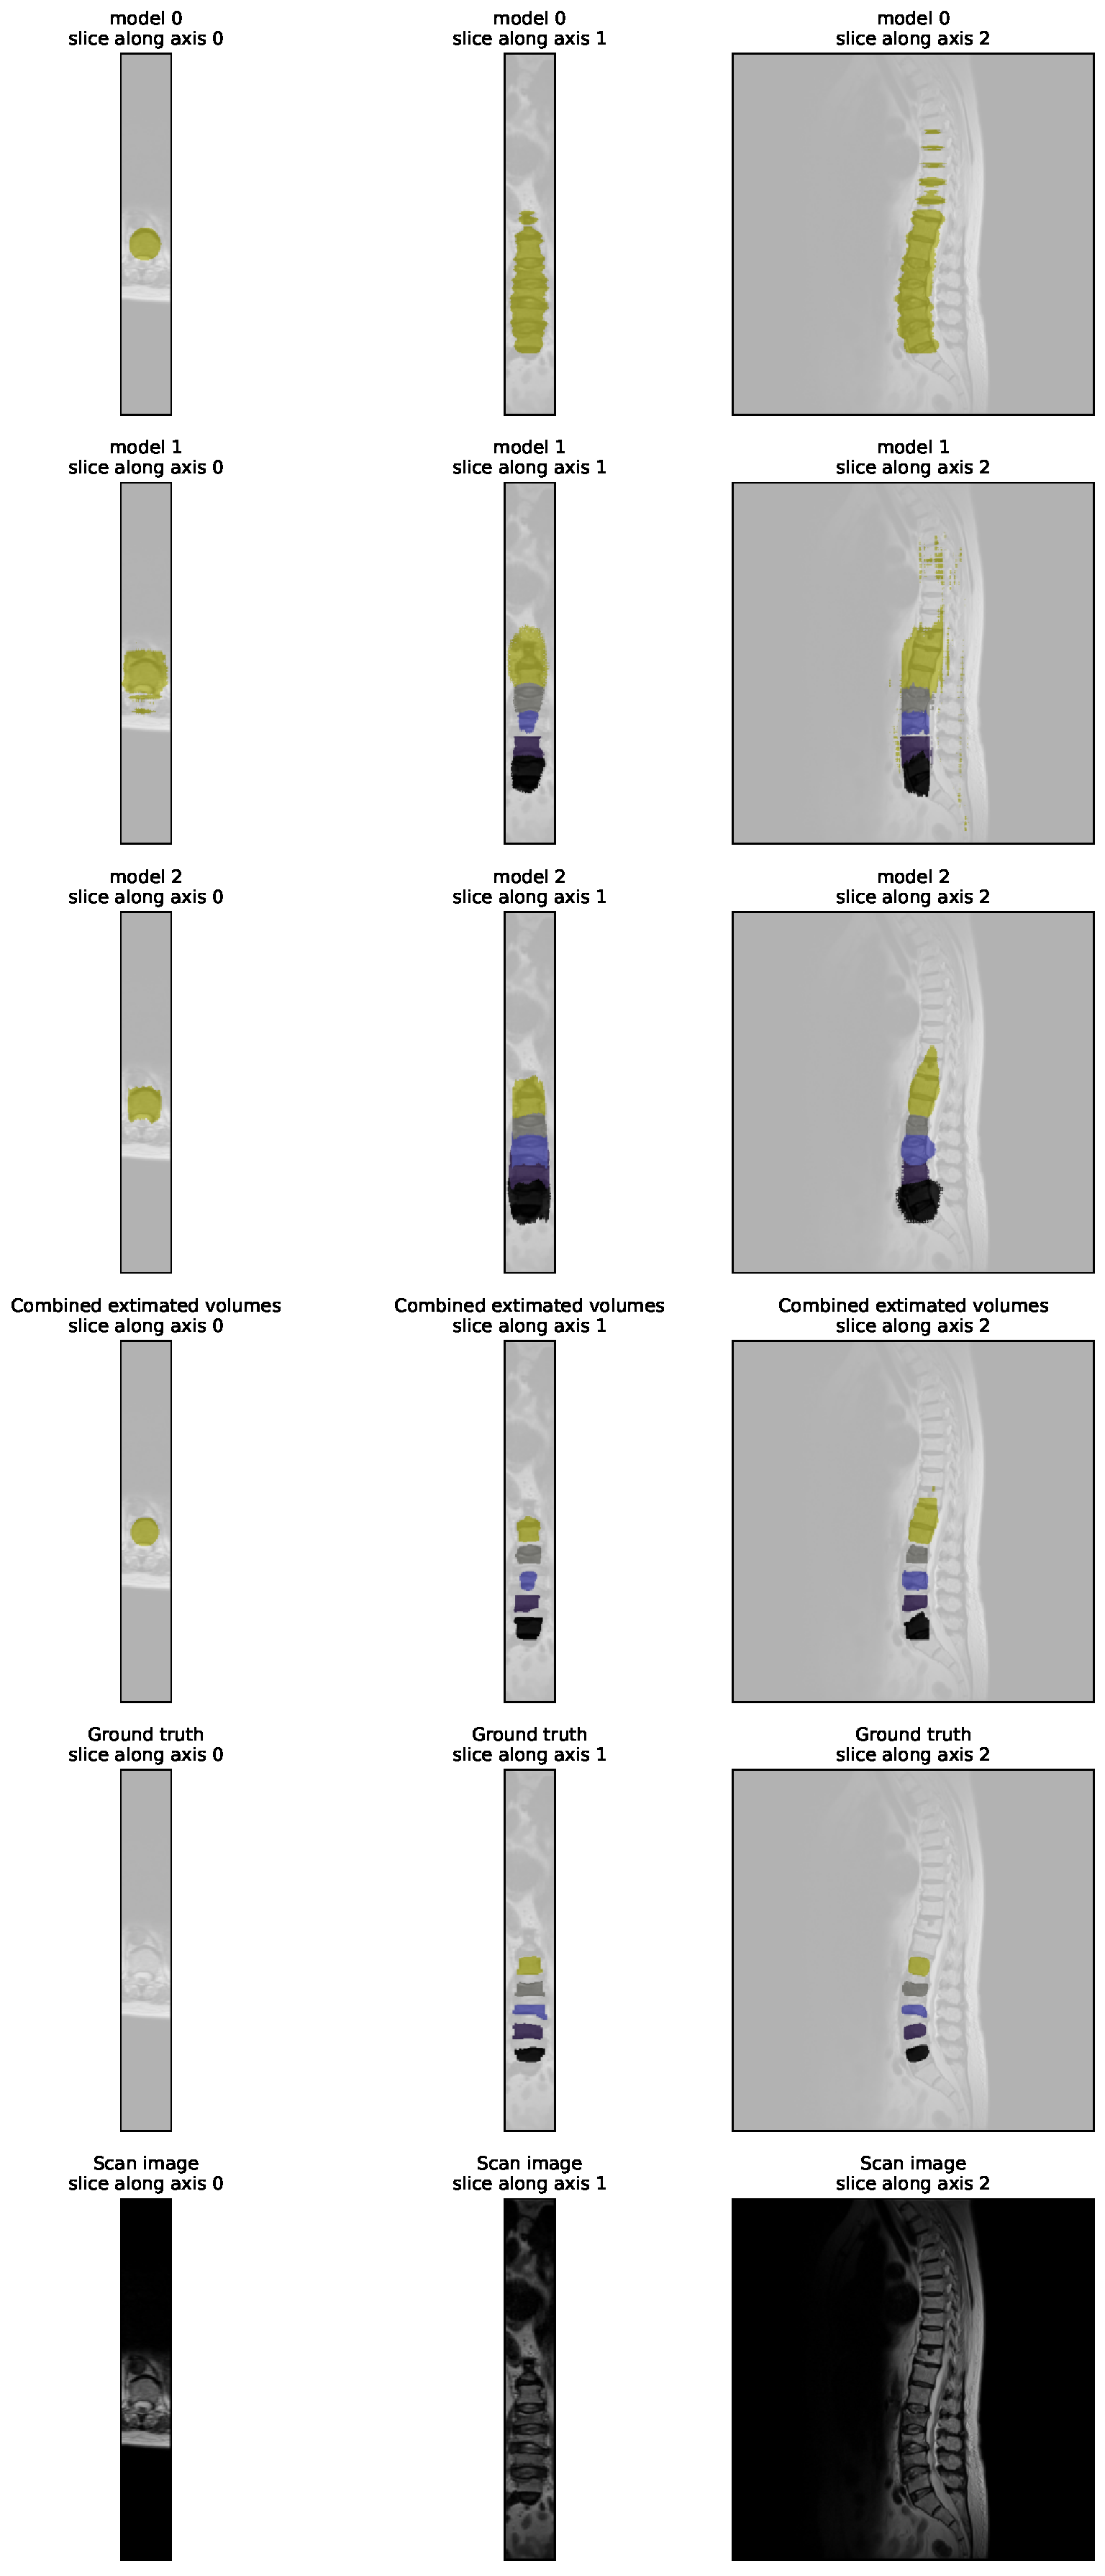
\includegraphics[width=.95\textwidth]{images/comb1_denoise2_erode1_USiegen_004.pdf}
    \caption{
        Result of the combination of the three single dimension model results for volume USiegen 004. The layout of this picture is identical to figure \ref{fig:comb1_1}.
        \protect\newline\noindent Colour legend: \newline
\noindent\mycircle{colL1}  L1 %\newline 
\hspace{2mm}\mycircle{colL2}  L2 %\newline 
\hspace{2mm}\mycircle{colL3}  L3 %\newline 
\hspace{2mm}\mycircle{colL4}  L4 %\newline 
\hspace{2mm}\mycircle{colL5}  L5
        \label{fig:comb1_3}
    }
\end{SCfigure}

\chapter{Pseudo mask training}
\par{
    In reality, an expert will generate a single stack of annotations, not three.
    As described in chapter \ref{sec:annotationPoints} on page \pageref{sec:annotationPoints}, one of the single dimensional models will be trained on this stack of annotated slices.
    The other two however, will be trained on stacks where the same annotation points are used, but now as these are found back when slicing in the two other dimensions.
    This means that for the slices along one of the geometric dimensions, a known number of annotation points will be provided.
    For the slices perpendicular to the other two geometric axis, the annotation points will have to be deduced from this original stack.
    Figures \ref{fig:inferepoints_1} and \ref{fig:inferepoints_2} illustrate this.
}
\marginpar{
        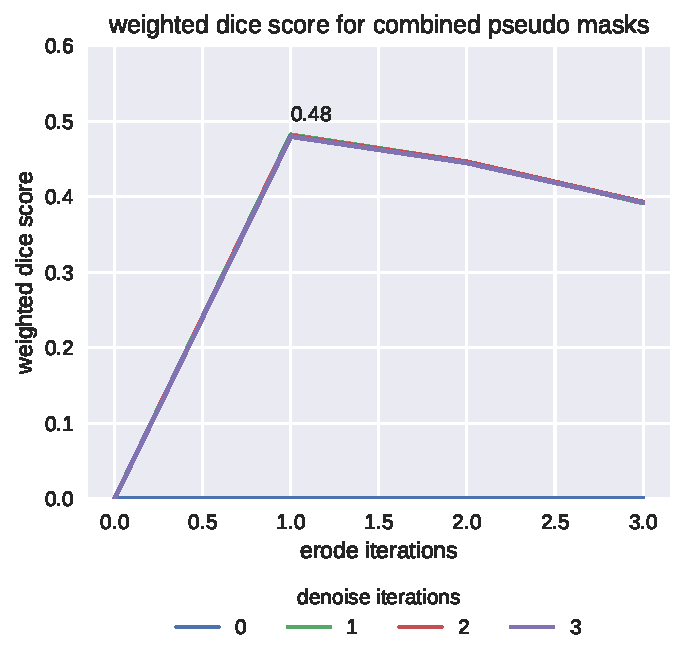
\includegraphics[width=5cm]{images/combination_optimization_precalc.pdf}
        \captionof{figure}{Illustration of the hyperparameter optimization procedure (see also table \ref{tab:combination_precalc})}
        \label{fig:hyperparameter_combination_precalc}
    }

    \marginpar{
        \begin{tabular}{l|ll}
            \textbf{\begin{tabular}[c]{@{}l@{}}labelled\\ \\ slices\end{tabular}} &
              \textbf{\begin{tabular}[c]{@{}l@{}}1 class pt\\ 1 BG pt\end{tabular}} &
              \textbf{\begin{tabular}[c]{@{}l@{}}3 class pt\\ 5 BG pt\end{tabular}} \\ \hline
            \textbf{transv.} & 4466 & 9121 \\
            \textbf{frontal}    & 2627 & 4507 \\
            \textbf{sagittal}   & 7939 & 7939
            \end{tabular}
        \captionof{table}{Available labelled slices from labelling the sagittal slice stack.}
    }
\par{
    Inferring annotation points from labels provided for slices taken in another direction implies the number of annotation points will vary.
    For some slices, no annotation points will be available.
    As a first test, point annotations in the sagittal slices with 1 class point per class instance and 1 background point were created.
    This showed to decrease the number of labelled strongly. When training with these slices, the segmentation networks showed to perform very poorly
    (inverse weighted dice scores of 0.22, 0.23 and 0.33 for the models trained respectively on the transverse, frontal and sagittal slice stacks).
    As is discussed on page \pageref{sec:trainingData} the cost of additional data points when the first point is provided is very low.
    When generating 3 labels per class instance and 5 background labels, the estimated cost is only increased to about $\frac{22,1 + 6.0,9}{239.7}=11,5\%$ of the cost of a full mask label.
    It is clear that this type of reasoning cannot be stretched to extremes (100 points or such), yet, the numbers of 3 and 5 seem perfectly reasonable.
}
\begin{SCfigure}[][htb]
    \centering
    \centering
    \begin{minipage}{.75\textwidth}
        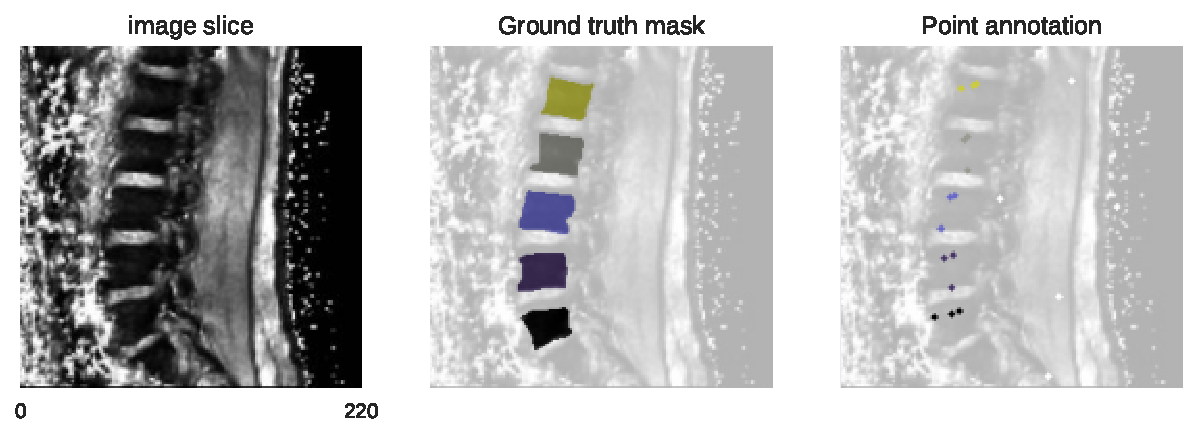
\includegraphics[width=.99\textwidth]{images/MyoSegmenTUM020_s21_points.pdf}
    \end{minipage} 
    \vspace{1 mm}
    \begin{minipage}{.75\textwidth}
        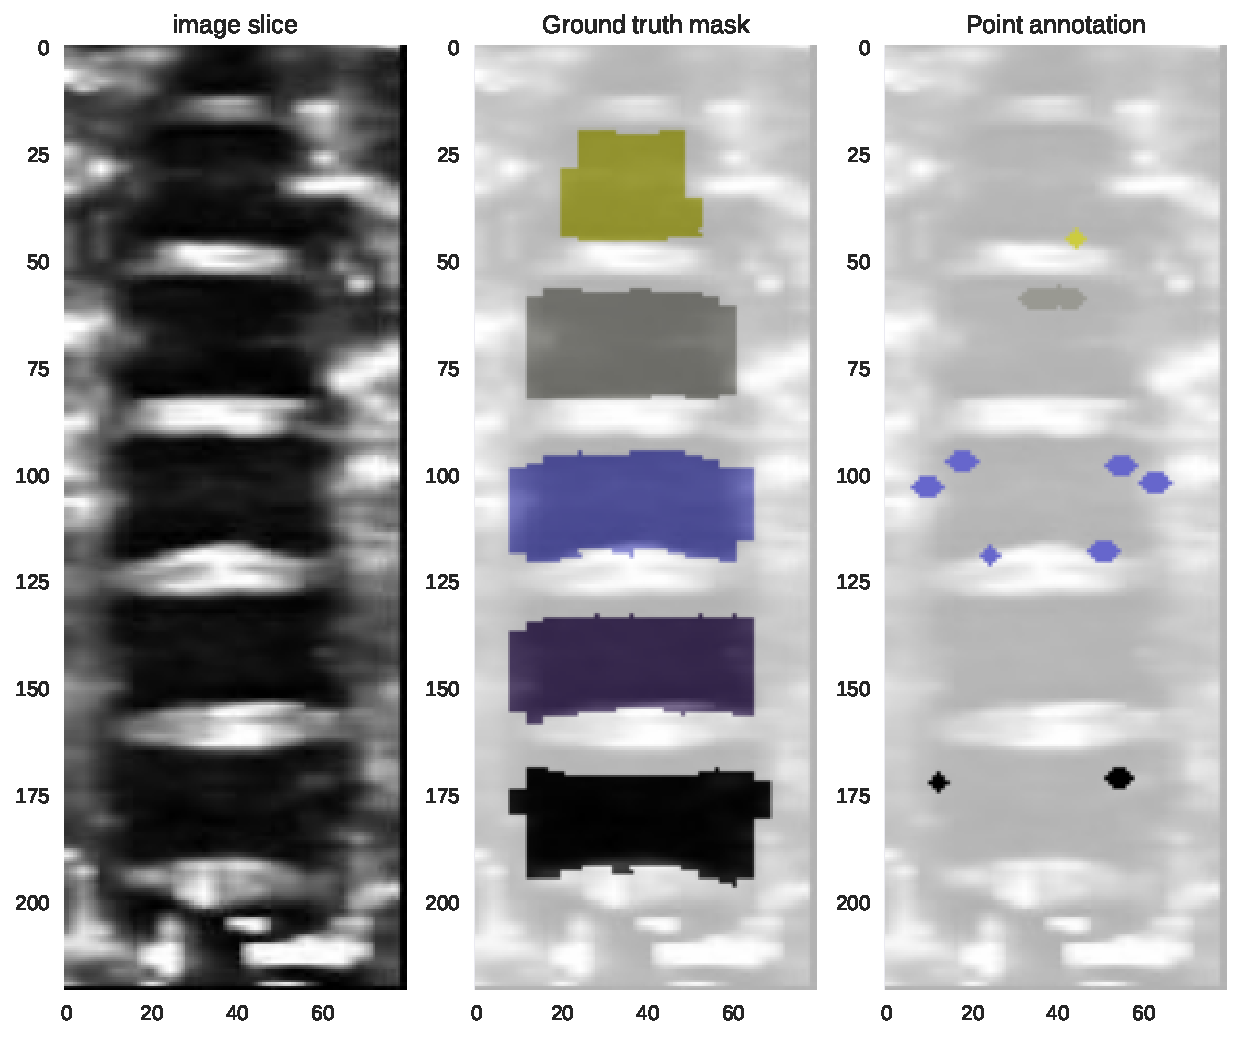
\includegraphics[width=.99\textwidth]{images/MyoSegmenTUM020_s75_front_points.pdf}
    \end{minipage} 
    \vspace{2 mm}
    \caption{Illustration of the single-stack labelling procedure.
    Since the labeller is only providing point annotations for the sagittal slices, slice 21 of MyoSegmenTUM 20 is labelled with the definded 3 class labels per class instance and 5 background point labels.
    The same annotation points show up in the frontal slice 75 of the same volume. 
    \protect\newline\noindent Colour legend: \newline
\noindent\mycircle{colL1}  L1 %\newline 
\hspace{2mm}\mycircle{colL2}  L2 %\newline 
\hspace{2mm}\mycircle{colL3}  L3 %\newline 
\hspace{2mm}\mycircle{colL4}  L4 %\newline 
\hspace{2mm}\mycircle{colL5}  L5\label{fig:inferepoints_1}}
\end{SCfigure}

\begin{SCfigure}[][htb]
    \centering
    \centering
    \begin{minipage}{.75\textwidth}
        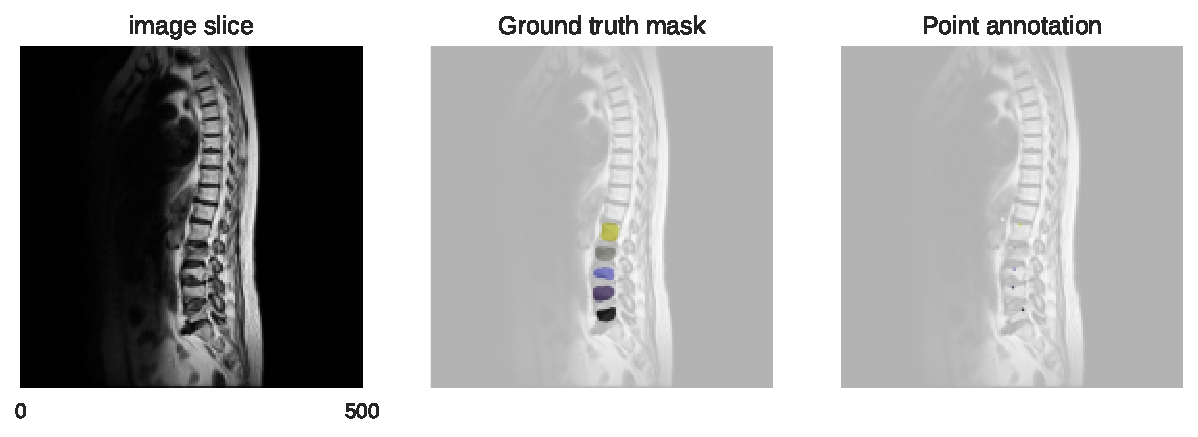
\includegraphics[width=.99\textwidth]{images/USiegen004_s20_points.pdf}
    \end{minipage} 
    \vspace{1 mm}
    \begin{minipage}{.75\textwidth}
        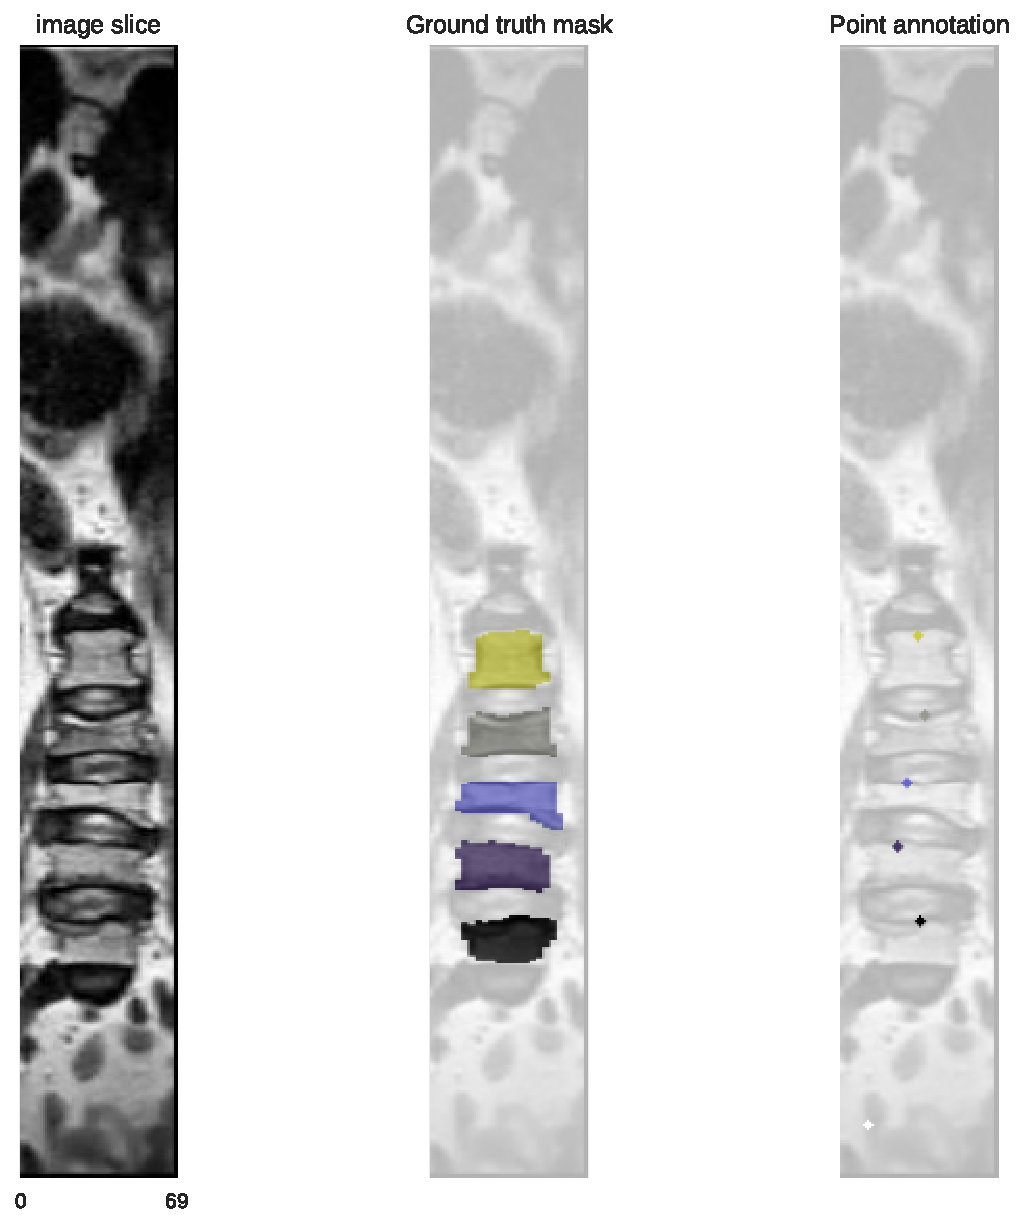
\includegraphics[width=.99\textwidth]{images/USiegen004_s250_front_points.pdf}
    \end{minipage} 
    \vspace{2 mm}
    \caption{Illustration of the single-stack labelling procedure.
    Since the labeller is only providing point annotations for the sagittal slices, slice 20 of USiegen 04 is labelled with the definded 3 class labels per class instance and 5 background point labels.
    The same annotation points show up in the frontal slice 250 of the same volume. 
    \protect\newline\noindent Colour legend: \newline
\noindent\mycircle{colL1}  L1 %\newline 
\hspace{2mm}\mycircle{colL2}  L2 %\newline 
\hspace{2mm}\mycircle{colL3}  L3 %\newline 
\hspace{2mm}\mycircle{colL4}  L4 %\newline 
\hspace{2mm}\mycircle{colL5}  L5\label{fig:inferepoints_2}}
\end{SCfigure}

% \begin{SCfigure}[][htb]
%     \centering
%     \centering
%     \begin{minipage}{.99\textwidth}
%         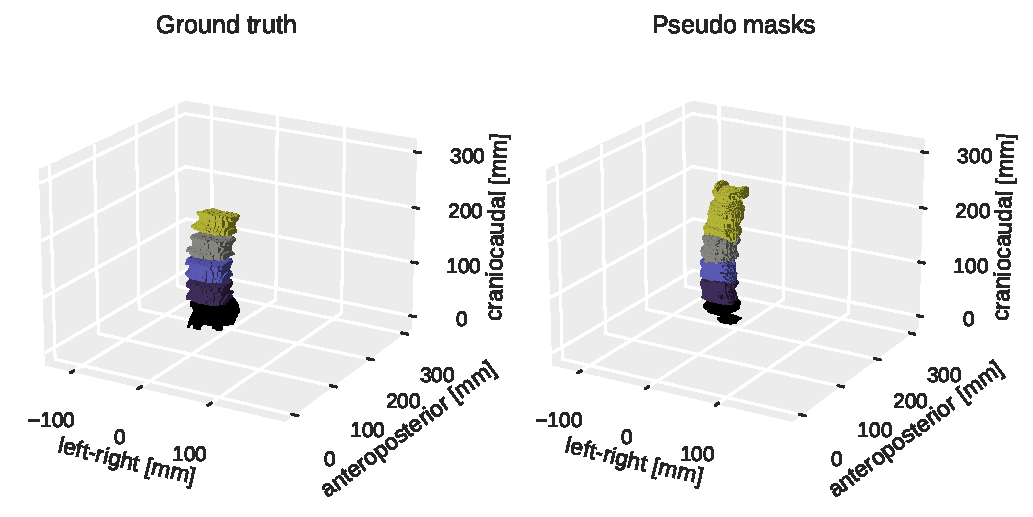
\includegraphics[width=.99\textwidth]{images/GroundTruth_morphComb_USiegen_007.pdf}
%     \end{minipage} 
%     \vspace{1 mm}
%     \begin{minipage}{.99\textwidth}
%         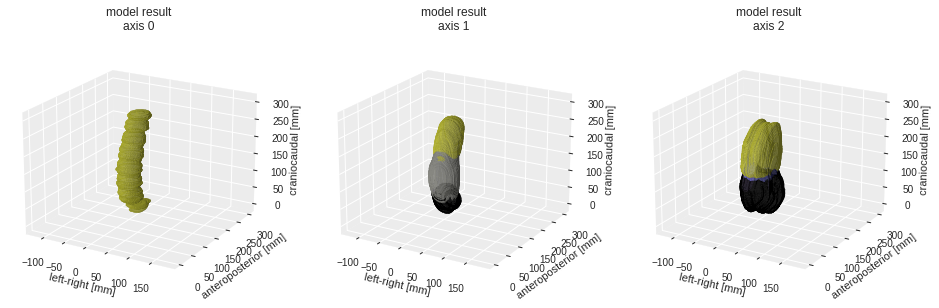
\includegraphics[width=.99\textwidth]{images/SingleDims_USiegen_007.pdf}
%     \end{minipage} 
%     \vspace{2 mm}
%     \caption{Thee dimensional render to visualize the combination of single-dimensional model results to form the pseudo masks.
%     The upper two figures show the ground truth volumes (as a reference, not used in training) and the pseudo mask volumes which have been constructed by comining the results of the three single dimensional models illustrated on the bottom row of images.
%     The scan illustrated here is USiegen 007.
%     \protect\newline\noindent Colour legend: \newline
\noindent\mycircle{colL1}  L1 %\newline 
\hspace{2mm}\mycircle{colL2}  L2 %\newline 
\hspace{2mm}\mycircle{colL3}  L3 %\newline 
\hspace{2mm}\mycircle{colL4}  L4 %\newline 
\hspace{2mm}\mycircle{colL5}  L5}
% \end{SCfigure}

% \begin{SCfigure}[][htb]
%     \centering
%     \centering
%     \begin{minipage}{.99\textwidth}
%         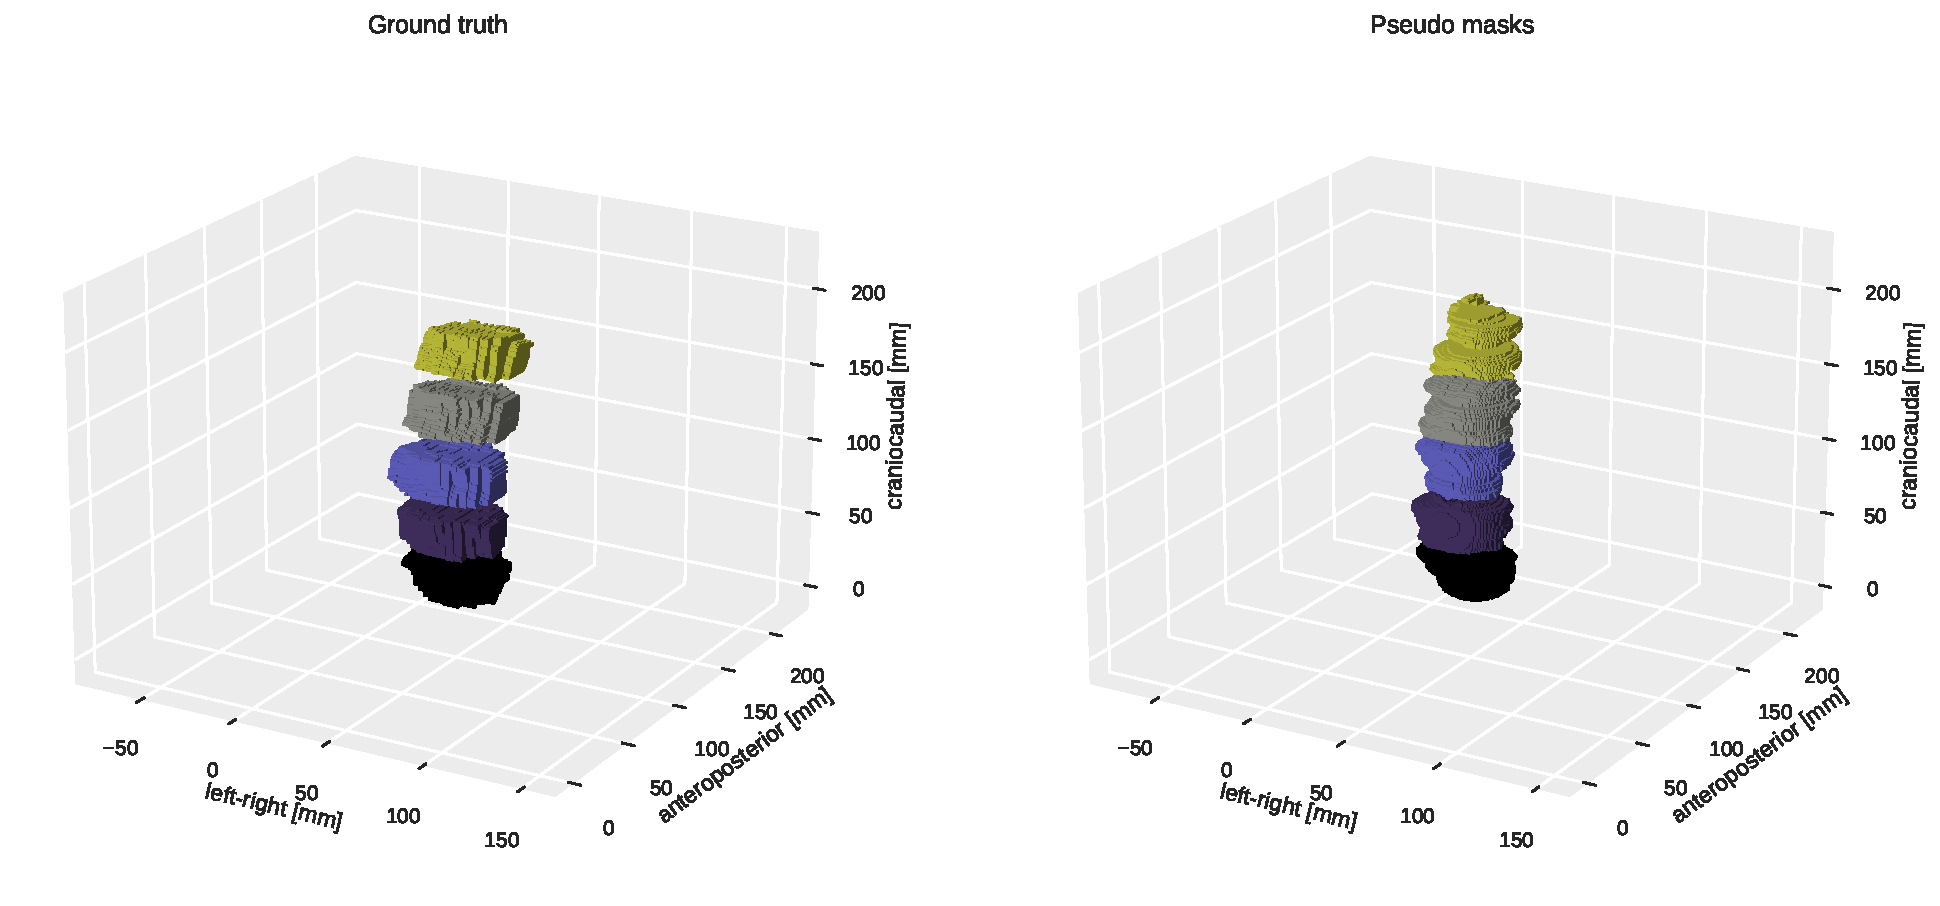
\includegraphics[width=.99\textwidth]{images/GroundTruth_morphComb_MyoSegmenTUM_034.pdf}
%     \end{minipage} 
%     \vspace{2 mm}
%     \begin{minipage}{.99\textwidth}
%         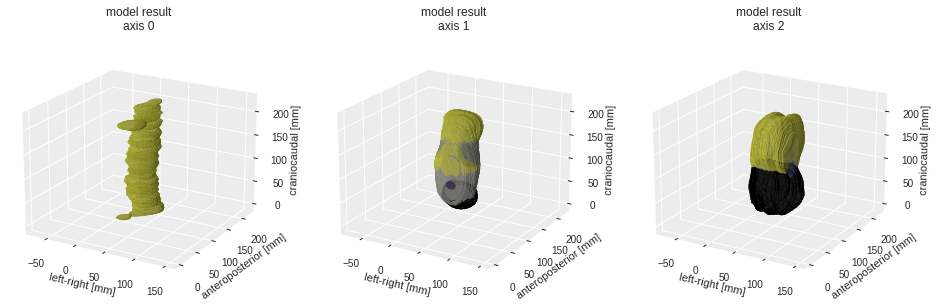
\includegraphics[width=.99\textwidth]{images/SingleDims_MyoSegmenTUM_034.pdf}
%     \end{minipage} 
%     \vspace{2 mm}
%     \caption{Thee dimensional render to visualize the combination of single-dimensional model results to form the pseudo masks.
%     The upper two figures show the ground truth volumes (as a reference, not used in training) and the pseudo mask volumes which have been constructed by comining the results of the three single dimensional models illustrated on the bottom row of images.
%     The scan illustrated here is MyoSegmenTUM 34.
%     \protect\newline\noindent Colour legend: \newline
\noindent\mycircle{colL1}  L1 %\newline 
\hspace{2mm}\mycircle{colL2}  L2 %\newline 
\hspace{2mm}\mycircle{colL3}  L3 %\newline 
\hspace{2mm}\mycircle{colL4}  L4 %\newline 
\hspace{2mm}\mycircle{colL5}  L5}
% \end{SCfigure}

Table \ref{tab:combination_precalc} illustrates how the performance of the combination of models trained on different slice stacks results in pseudo masks which prove to be an improvement compared to the individual models.
It is remarkable how high the performance of the models trained on \textit{inferred} annotation points proves to be.
Seemingly, randomizing the number of annotation points could have a positive influence on the model performance.

\begin{SCtable}[\sidecaptionrelwidth][h]

    \begin{tabular}{l|lll}
        \hline
        \textbf{\begin{tabular}[c]{@{}l@{}}Slice \\ direction\end{tabular}} &
          \textbf{Transverse} &
          \textbf{Coronal} &
          \textbf{Sagittal} \\ \hline
        \begin{tabular}[c]{@{}l@{}}Context\\ Slices {[}mm{]}\end{tabular}           & 1        & 1        & 1    \\ \cline{1-1}
        \begin{tabular}[c]{@{}l@{}}Points per\\ class instance\end{tabular}         & variable & variable & 3    \\ \cline{1-1}
        \begin{tabular}[c]{@{}l@{}}Background \\ points\end{tabular}                & variable & variable & 5    \\ \cline{1-1}
        Dataset &
          \begin{tabular}[c]{@{}l@{}}PLoS\\ xVertSeg\\ USiegen\\ MyoSegmenTUM\end{tabular} &
          \multicolumn{2}{l}{\begin{tabular}[c]{@{}l@{}}xVertSeg\\ USiegen\\ MyoSegmenTUM\end{tabular}} \\ \cline{1-1}
        \begin{tabular}[c]{@{}l@{}}Segmentation\\ classes\end{tabular}              & 2        & 6        & 6    \\ \cline{1-1}
        \begin{tabular}[c]{@{}l@{}}score \\ $dice_{wi}$\end{tabular}              & 0.51     & 0.41     & 0.34 \\ \hline
        \begin{tabular}[c]{@{}l@{}}score \\ $dice_{wi}$\ combination\end{tabular} & \multicolumn{3}{c}{0.48}   \\ \hline
        \end{tabular}
    \caption{Combination of three point supervised models with algorithm \ref{alg:combination}. 
    These models were constructed from points labels that were provided on the sagittal slice stack.
    The labels for the other two slice stacks were derived from this first one.
    This test indicates that the segmentation mask obtained from the result of single dimension models with algorithm \ref{alg:combination} allows to obtain a new segmentation mask with a higher metric score, the pseudo masks.
    The weighted dice scores are evaluated on the cross validation set, this causes the difference with the values in figure \ref{fig:points_influence} where the values were obtained by evaluation on the test set. \label{tab:combination_precalc}
    }

\end{SCtable}

\FloatBarrier

Illustration \ref{fig:fullvsPseudo} shows the final result of the procedure.
With the pseudo masks obtained from combining the three model results, a new model is trained.
This last model is only trained on the sagittal slice stack.
The final results obtained with this model are illustrated in figure \ref{fig:fullvsPseudo}.
The hyperparameters of this model were optimized in the same way as the reference model.
It is remarkable that for this model, the weighted cross entropy loss proves to yield better results than the non-weighted cross entropy loss.
For the reference model, the opposite result was observed.

The confusion matrix of the model trained with pseudo mask labels (table \ref{tab:pseudo_confusionMatrix}) shows the model performance is clearly inferiour to the model performance of the fully supervised model.
Mind however that this model is trained based on data of which the labelling only costs about 12\% of the labelling cost of the fully supervised model for the train set scans.
The total labelling cost will be higher since the procedure requires full labels for the model evaluation in the cross validation and the test set. 
If one takes, is was done in this thesis, both the cross validation and test set to be $\frac{1}{6}$ of the total volumes, the total cost is about 41 \% of the cost for full labels.
One could also look at it in another way: for fixed cross validation and test set, the train set can be made 8,3$\times$ larger with the same labelled cost.


\begin{SCfigure}[][htb]
    \centering
    \begin{minipage}{.99\textwidth}
        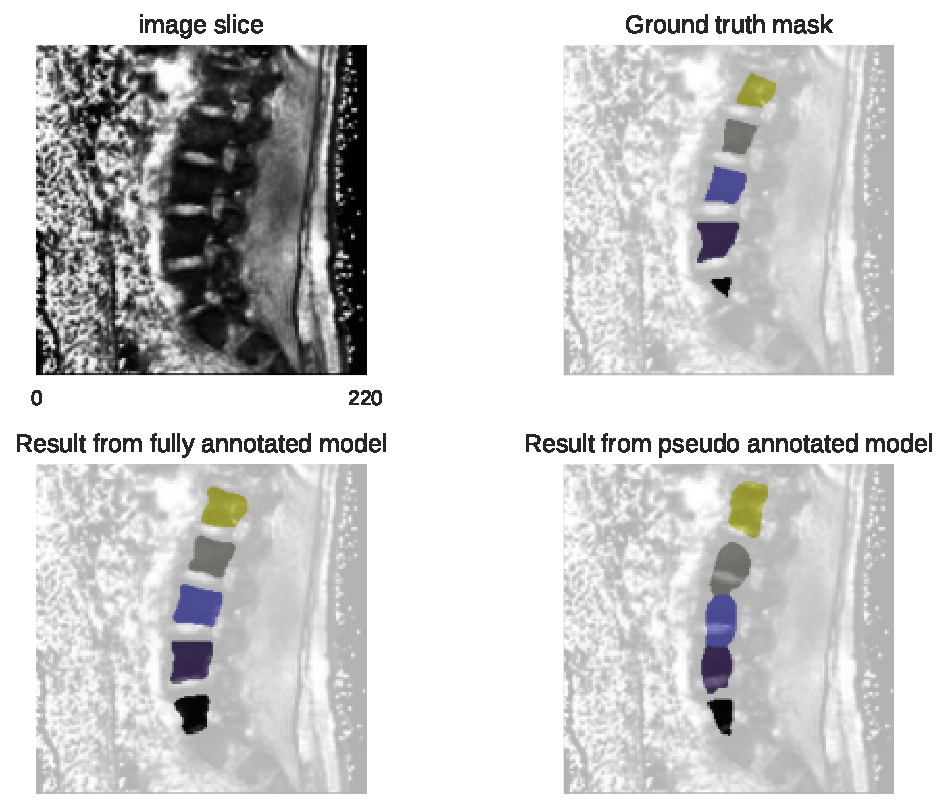
\includegraphics[width=.99\textwidth]{images/fullvsPseudo_MyoSegmenTUM_024_023.pdf}
    \end{minipage} 
    \vspace{2 mm}
    \begin{minipage}{.99\textwidth}
        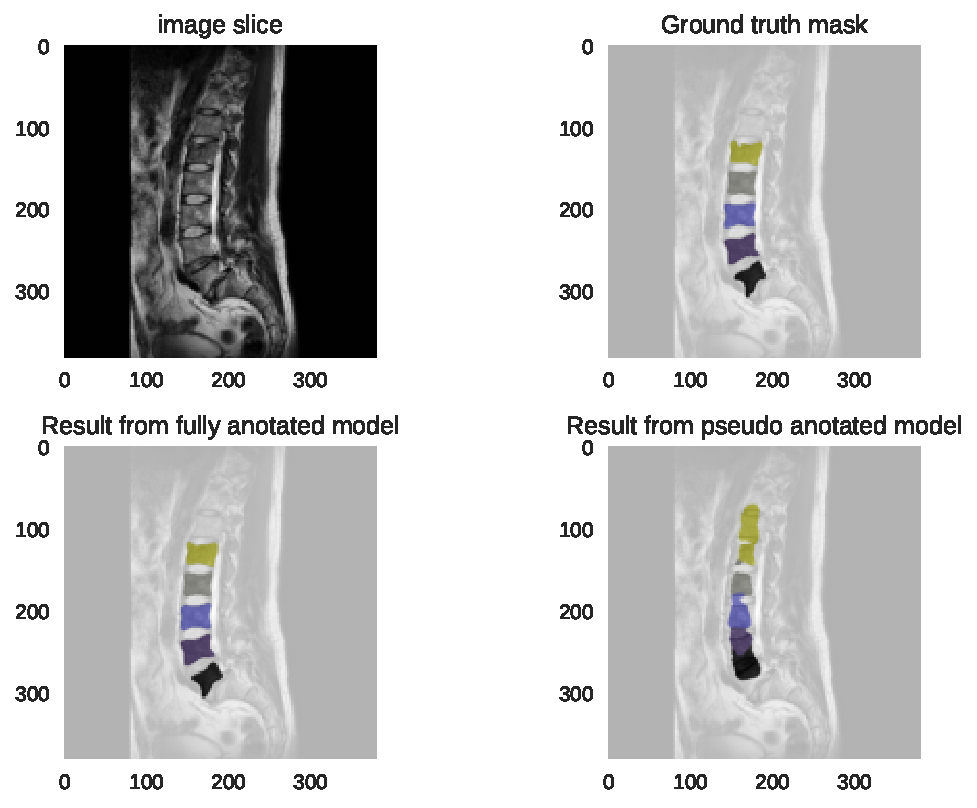
\includegraphics[width=.99\textwidth]{images/fullvsPseudo_USiegen_012_024.pdf}
    \end{minipage} 
    \vspace{2 mm}
    \begin{minipage}{.99\textwidth}
        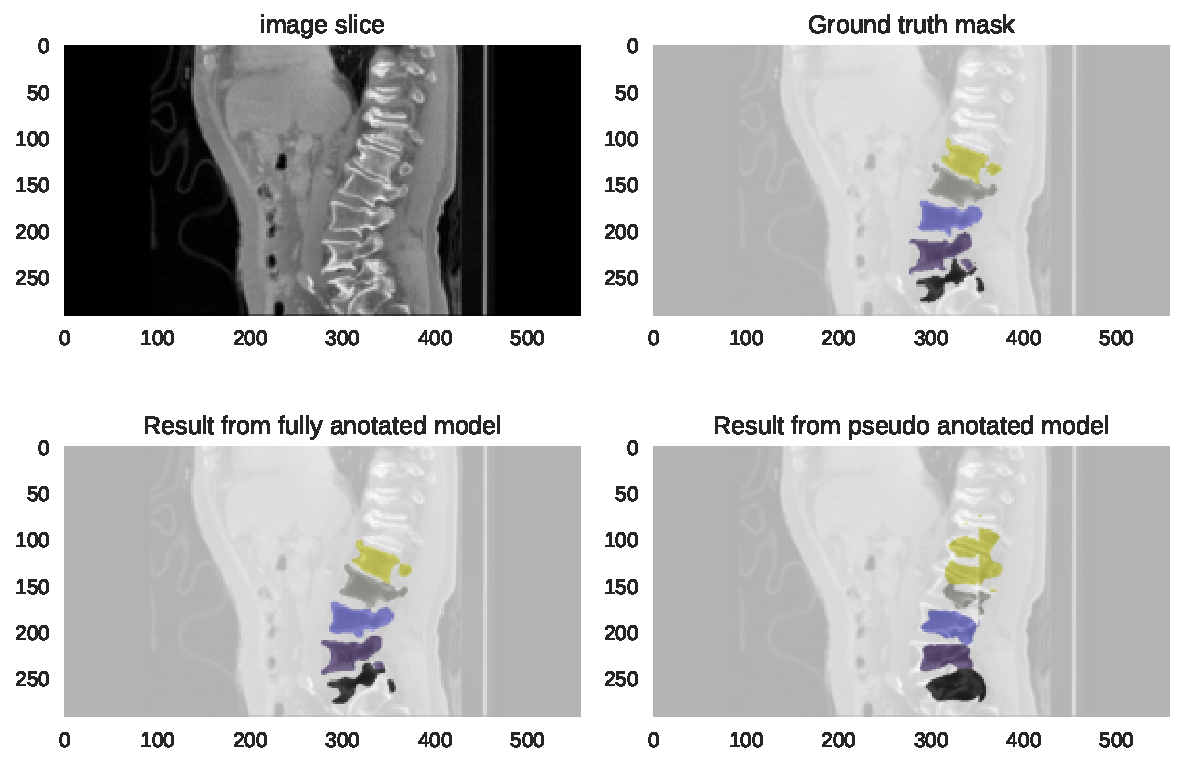
\includegraphics[width=.99\textwidth]{images/fullvsPseudo_xVertSeg_014_260.pdf}
    \end{minipage}
    \caption{These images illustrate the difference in performance for the two models generated. On the top row, an image slice is shown next to the ground truth annotation mask.
    Two models were trained: the reference model, shown left on the second row and a model trained on pseudo masks of which the result is shown on the right side. 
    These images show the final result of the procedure described in this thesis. The shown masks are not the pseudo masks themselves, they are the results obtained from the final model trained on these pseudo masks.
    From top to bottom, the image shows these results for slice 23 of MyoSegmenTUM volume 24, slice 24 of USiegen volume 12 and slice 260 of xVertSeg volume 14. 
    \protect\newline\noindent Colour legend: \newline
\noindent\mycircle{colL1}  L1 %\newline 
\hspace{2mm}\mycircle{colL2}  L2 %\newline 
\hspace{2mm}\mycircle{colL3}  L3 %\newline 
\hspace{2mm}\mycircle{colL4}  L4 %\newline 
\hspace{2mm}\mycircle{colL5}  L5
    \label{fig:fullvsPseudo}}
\end{SCfigure}

\begin{SCtable}[\sidecaptionrelwidth][h]
 
    % Please add the following required packages to your document preamble:
% \usepackage{multirow}
% Please add the following required packages to your document preamble:
% \usepackage{multirow}

\begin{tabular}{cl|llllll}
    \toprule
    \multicolumn{2}{l|}{\multirow{2}{*}{values in {[}\%{]}}} & \multicolumn{6}{c}{\textbf{Predicted}}                                            \\
    \multicolumn{2}{l|}{}                                    & \textbf{BG} & \textbf{L1} & \textbf{L2} & \textbf{L3} & \textbf{L4} & \textbf{L5} \\ \hline
    \multirow{6}{*}{\textbf{Actual}}      & \textbf{BG}      & 99.5        & 85.39        & 23.63        & 25.36        & 24.87        & 41.04        \\
     & \textbf{L1} & 0.09 & 59.87 & 2.96  & 0.07  & 0  & 0    \\
     & \textbf{L2} & 0.11 & 5.68  & 50.22 & 2.08  & 0  & 0    \\
     & \textbf{L3} & 0.11 & 0    & 2.46  & 54.57 & 2.48  & 0    \\
     & \textbf{L4} & 0.11 & 0    & 0    & 3.87    & 56.09 & 1.81  \\
     & \textbf{L5} & 0.11 & 0.05    & 0    & 0    & 1.67  & 55.07 \\ \bottomrule
    \end{tabular}

    \caption{Confusion matrix for the model trained with pseudo label masks (network VGG16-FCN8 and cross-correlation loss), evaluated on the test set.
    The values have been normalized by the total number of voxels classified in each class.
    \label{tab:pseudo_confusionMatrix}
    }
\end{SCtable}

\marginpar{
        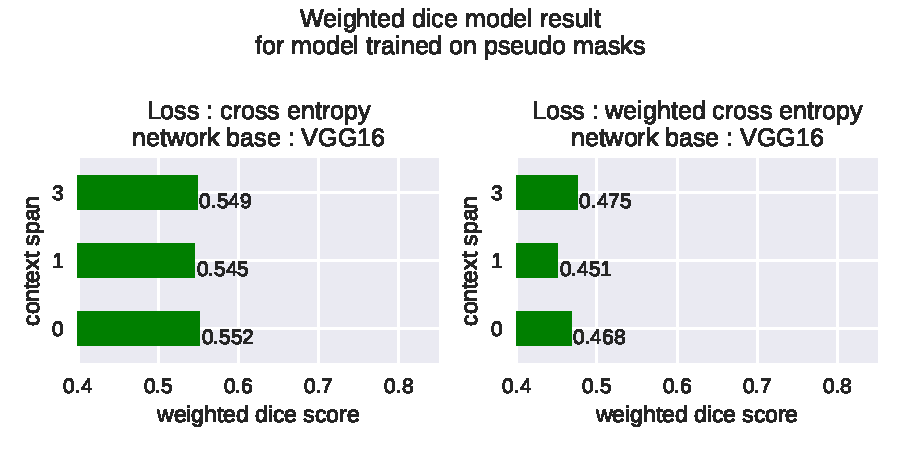
\includegraphics[width=5cm]{images/PseudoSupervised.pdf}
        \captionof{figure}{Class-weighted dice score for models trained on pseudo-masks. }
        \label{fig:PseudoSupervised_dice}
    }

Since the final model is exactly the same network as the reference model, only trianed with pseudo masks instead of full masks, the inference time is exactly the same.
To preproces the 105 images in the 4 datasets used for training, 


\begin{SCtable}[\sidecaptionrelwidth][h]

    % Please add the following required packages to your document preamble:
% \usepackage{multirow}
\begin{tabular}{ll|lllll}
\hline
\multicolumn{2}{l}{\multirow{2}{*}{Weighted dice score}}               & \multicolumn{5}{c|}{Trained and evaluated on} \\
\multicolumn{2}{l}{} &
    all datasets &
    \begin{tabular}[c]{@{}l@{}}MyoSegmenTUM \\ only\end{tabular} &
    \begin{tabular}[c]{@{}l@{}}USiegen\\ only\end{tabular} &
    \begin{tabular}[c]{@{}l@{}}xVertSeg\\ only\end{tabular} &
    \begin{tabular}[c]{@{}l@{}}PLoS \\ only\end{tabular} \\ \hline
Reference                                                   &          & 0.76     & 0.00     & .000    & 00      &     \\ \hline
\multirow{3}{*}{\begin{tabular}[c]{@{}l@{}}Single-\\ dimension models\\ with annotation\\ poins on sagittal\\ slices\end{tabular}} &
    Transverse &
    0.53 &
    0.64 &
    0.71 &
    0.62 &
    0.70 \\
                                                            & Frontal  & 0.41     & 0.46     & 0.37    & 0.41    &     \\
                                                            & Sagittal & 0.34     & 0.36     & 0.28    & 0.36    &     \\ \hline
\begin{tabular}[c]{@{}l@{}}Pseudo mask\\ model\end{tabular} &          & 0.55     & 0.00     & 0.00    & .000    &     \\ \hline
\end{tabular}
    \caption{Summary
    }

\end{SCtable}